\section{Relevant Model Details}

The HuMoR architecture is that of a C-VAE \cite{CVAE}, as can be seen in \figref{fig:humor_architecture}. The goal of this architecture is to learn a mapping from a given pose ($\textbf{x_{t-1}}$) to a distribution over latent transitions to the next pose  (the $\textbf{\textcolor{orange}{prior}}$), and a mapping from a latent transition sampled from this distribution to a change in pose that can be used to obtain the next state ($\textbf{\textcolor{blue}{decoder}}$). This is achieved during training through additional $\textbf{\textcolor{green}{encoder}}$ network that has the full information of the next state ($\textbf{x_t}$) also available to it, such that it can find the ideal latent transition, and this is used to guide the training of the $\textbf{\textcolor{orange}{prior}}$ network.

\begin{figure}[!ht]
    \centering
    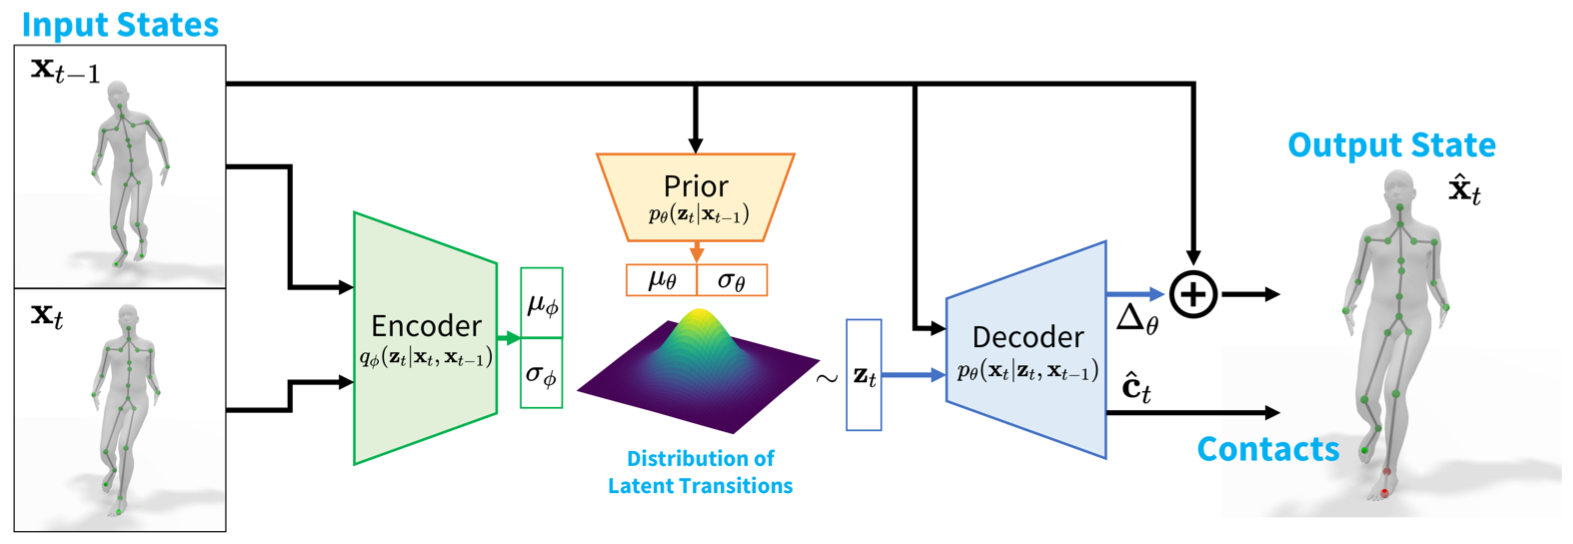
\includegraphics[width=1\textwidth]{Figures/humor/model/architecture.png}
    \caption{HuMoR C-VAE Architecture}
    \label{fig:humor_architecture}
\end{figure}


\TODO{Describe the model in more detail, include architecture diagrams etc., describe the rollout and the various stages of the model}
